%% Note that anything in a LaTeX file which is preceded (on the same line)
%% by a % is a comment, and is totally ignored by LaTeX.

%\documentclass[aps,prd,preprint]{revtex4}
\documentclass[aps,prd,final,twocolumn,letterpaper]{revtex4}
\usepackage{amsfonts}
\usepackage{tcolorbox}


% Note:  comment out one of the two documentclass commands, depending
% on whether you need the final or preprint version. It is most convenient
% to work in preprint mode, and switch to final only at the end.

\usepackage{graphicx}                            % Graphics package
\usepackage{epstopdf}
\usepackage{amsmath} 


%% The next few lines are definitions of commands used by Prof. Jaffe
%% when he wrote his paper.  The LaTeX-sophisticated among you
%% may have defined some labor-saving commands of your own.
%% If so, they go here.  The LaTeX-unsophisticated among you
%% may nevertheless want to use some of Prof. Jaffe's commands,
%% like \bra and \ket and \braket,  as done in the template below.
%% If you use these commands in your paper, keep their definitions
%% here.  If you do not use them, you can delete them.

\newcommand{\sech}{\mathop{\rm sech}\nolimits}
\newcommand{\bra}[1]{\left\langle #1 \right|}
\newcommand{\ket}[1]{\left|#1\right\rangle}
\newcommand{\braket}[2]{\left\langle#1 |  #2\right\rangle}
\newcommand{\rd}[1]{\mathop{\mathrm{d}#1}}


%%%%%%%%%%%%%%%


\begin{document}


%%%%%%%%%%%%%%
%%
%% Now, the document itself begins.  When you are ready to begin writing
%% your own paper, you will cut content out of the following and
%% replace it with your own.  Keep an unmodified copy of this
%% LaTeX file, though, and a hard copy of the paper by Prof.
%% Jaffe which it produces.  Comparing the template below with
%% the hard copy it produces will help you see how to handle
%% titles, sections, figures, equations, references, the bibliography
%% and much more.  Good luck with your paper. JN.
%%
%%%%%%%%%%%%%%

\title{Cipher Breaking using Markov Chain Monte Carlo}
\author{Thiago~R.~Bergamaschi}
\affiliation{ Center for Theoretical Physics,
 77 Massachusetts Ave.,
Cambridge, MA 02139-4307}
\date{\today} 

\begin{abstract}
\noindent	
This is my report of Part 2 of the 6.437 final project in Spring 2019. We first implemented a Markov Chain to break a substitution Cipher encryption, and then refined our analysis in part 2. In particular, I propose 2 enhancements: Ensemble MCMC, i.e. running multiple walks on the MC in parallel, and initialization by linear assignment. We also adapt the search for the existence of a breakpoint in the ciphertext.
\end{abstract}

\maketitle
\pagestyle{myheadings}
\markboth{Thiago R. Bergamaschi}{6.437 Project Part 2}
\thispagestyle{empty}


\section{Introduction}
A substitution cipher is a method of encryption by which units of plaintext the original message are replaced with ciphertext the encrypted message according to a ciphering function, e.g. some permutation of the alphabet $A = \{a, b, \cdots, z\}\cup \{\ ., \}$. 

Given apriori probabilities for the letters in the english language, $p_a(i)=\mathbb{P}[i]$ for $i\in A$, and bigram transition probabilities, $M_{ij}=\mathbb{P}[x_{k} = i|x_{k-1} = j]$, there is a closed form expression for the likelihood of the observed ciphertext $\mathbf{y}$ for a given permutation $f$.

\begin{equation}
p_{\mathbf{y}|f}(\mathbf{y}|f) =  p_a(f^{-1}(y_1))\times \prod_{i=1} \mathbb{P}[f^{-1}(y_{i+1}) |f^{-1}(x_{i})]
\end{equation}

For part 1 of this project, we implement a simple Markov Chain on the set of possible permutations. This approach is shown in section 2 of the report, where we discuss and test general implementation enhancements as well. In section 3, we describe the algorithmic enhancements used in part 2. In particular, running multiple ($N = 5$ typically) walks on the Markov Chain and returning the maximum decreases the failure probability considerably, at little to no increase in runtime. Next, we improve on the permutation initialization by linear assignment. We define costs for each swap $ij$ of the permutation, based on the a priori probability of $i$ in the English language, and the empirical probability of $j$ in the ciphertext, and solve the assignment problem with the Hungarian algorithm. Finally, in section 4, we adapt our implementation for the existence of a breakpoint in the ciphertext.


\section{Markov Chain Monte Carlo}
Given these likelihoods, we can construct a Markov Chain on the set of possible permutations. Define edges between permutations that swap a pair of letters. At each vertex $f$, we pick one of $\binom{28}{2}$ adjacent edges $f'$, and transition there with probability
\begin{equation}
\min\{1, \frac{p_{\mathbf{y}|f}(\mathbf{y}|f')}{p_{\mathbf{y}|f}(\mathbf{y}|f)}\}
\end{equation}

The algorithmic description follows.\\

\noindent \textbf{Input:} alphabet $A$, ciphertext $\mathbf{y}$, iteration number $T$.
\noindent\textbf{Output:} most probable permutation $f_p$



\begin{enumerate}
\item initialize $f$ with some random permutation of $A$, and iteration count $t=0$. Compute $p_{\mathbf{y}|f}(\mathbf{y}|f)$.
\item While $t<T$, construct $f'$ by swapping 2 letters of $f$, and compute $p_{\mathbf{y}|f}(\mathbf{y}|f')$.
\item Pick a random $x\in [0, 1]$. If $\frac{p_{\mathbf{y}|f}(\mathbf{y}|f')}{p_{\mathbf{y}|f}(\mathbf{y}|f)}> x, f\leftarrow f'$.
\item $t\leftarrow t + 1$, repeat step 2.
\item Return $f$.
\end{enumerate}

Clearly, there is immediate space for improvement by speeding up the $p_{\mathbf{y}|f}(\mathbf{y}|f)$ computation. Some of the performance enhancements include defining a less memory intensive sufficient statistic, quickly computing loglikelihoods, and perturbing the 0 transition probabilities s.t. the loglikelihoods are strictly finite.

\subsection{Performance Enhancements}
Note first that we can compute the log likelihood $\log p_{\mathbf{y}|f}(\mathbf{y}|f)$ from $\log p_a(f^{-1}(y))$, and the count matrix $C$ where $c_{ij}$ is the number of times $j$ is preceded by $i$ in $y$. It follows 
\begin{equation}
\log p_{\mathbf{y}|f}(\mathbf{y}|f) = \log p_a(f^{-1}(y)) + \sum_{ij} c_{ij}\log M_{f(i)f(j)}
\end{equation}

\noindent and thus $C,p_a(\cdot)$ is a sufficient statistic for our model. 

Moreover, we can precompute $C$ in $O(\text{text size})$ and compute the loglikelihood as in (3), instead of passing through the text at every vertex. 

Finally, note that if we initialize the MCMC at some permutation $f$ that implies $p_{\mathbf{y}|f}(\mathbf{y}|f) = 0$ due to some 0 valued $M_{ij}$, then the loglikelihood value will be $-\infty$. More importantly, empirical evidence suggests that randomly initializing $f$ sets a considerable probability of failure, due to taking a long time to leave this minima. We easily fix this by assigning large, finite, negative values to the values of $\log M_{ij}$ when $M_{ij} = 0$. In particular, $-2000$ was found to work well.

\subsection{Results of Part 1}
To briefly comment on current performance, a \textit{single pass }of the MCMC when successful runs $3000$ iterations in $\approx 5s$ and decoding accuracy $\approx .97$. However, due to faulty initialization and general convergence issues, it is only successful about $\frac{2}{3}$ of the time. The following plot shows the convergence of the current permutation log likelihood as function of iteration.

\begin{figure}[h]
\centering
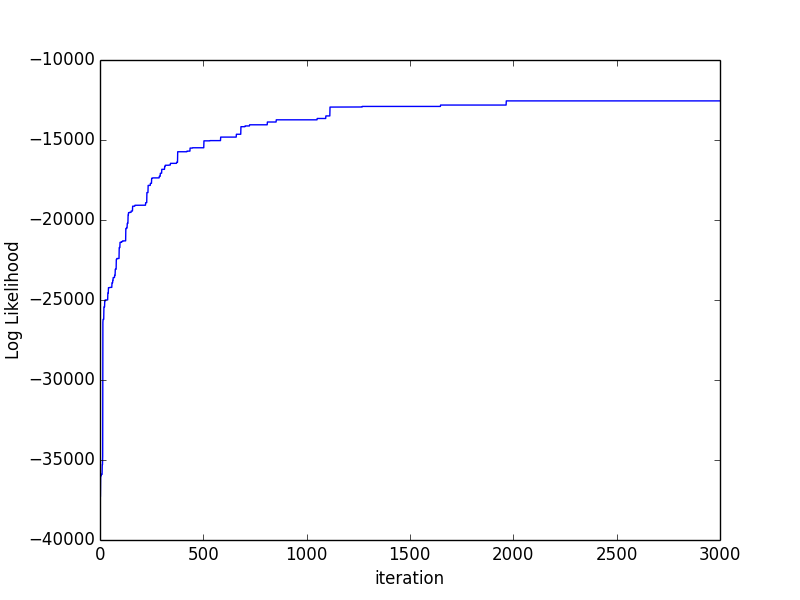
\includegraphics[scale=.3]{logl.png}
\caption{Log Likelihood as function of number of Iterations}
\end{figure}

As of part 1, we can guarantee fault tolerance, and larger accuracy at the cost of runtime by sequentially repeating, and taking the maximum returned log likelihoods. We hope to build on the accuracy in part 2.

\section{Algorithmic Enhancements}
We suggest 2 main algorithmic enhancements. The first is to run multiple threads/walks in parallel, and take the maximum among them. The second is to build on the initialization to guarantee a non zero (or non-negligible) initial accuracy. We do so as a linear assignment problem, matching the a priori probabilities $p_a(\cdot)$ with the empirical frequencies $q_{a'}(\cdot)$ in the cipher, thereby matching each $a$ with an $a'$. 

We introduce a performance improvement as well. Empirical evidence suggests the log of the likelihood ratio is typically has large absolute value. So, instead on generating random $x\in[0, 1]$ to define the acceptance (2), we just condition on the log of the likelihood ratio to be positive. This slightly increases runtime.



\subsection{Initialization}
We construct a bipartite graph $[|A|]\cup [|A|]$ corresponding to matching the alphabet to a permutation. We set costs $V_{ij} = (p_a(i)-q_{a'}(j))^2$, defining a cost matrix $V$. We then run the Hungarian algorithm to find a min cost perfect matching, returning a permutation of $A$. This allows us to initialize each MCMC with a permutation with initial accuracy $\approx .45 \pm .05$. A thorough algorithmic description can be found in [1].

\subsection{Multiple Walks}
As of part 3.A, one pass of our MCMC runs 7000 iterations in approximately $6\pm 1$s, and has average accuracy .999 when successful, .84 overall. When we use $\geq 3$ threads or sequential repetitions, each running an MCMC on 7000 iterations, the overall accuracy increases to .999.



\section{Breakpoint}
We find the breakpoint within $n/200$th characters by binary search for the maximum loglikelihood position. In particular, for each possible breakpoint position $x$, we run the MCMC on the first $x$ characters and the remaining $n-x$, and sum their loglikelihoods. If the loglikelihood is larger than the loglikelihood at $x-\frac{n}{100}$, then we recursively search in the right half, and vice versa. This runs in $\geq \log_2 100$ recursive steps, each calls twice the algorithm in part 3. The runtime is approximately 500s, for a .993 average accuracy.

\section{Conclusion}
In this report, I comment on my refinements to the MCMC approach in part 1 with 2 algorithmic improvements, parallelization and guaranteed initialization with linear assignment. In section 2, I briefly present algorithm used, and the implementation details in part 1. Finally, I describe my approach to the breakpoint problem in section 4.





\end{document}
